                             %%%%%%%%%%%%%%%%%%%%%%%%%%%%%%%%%%%%%%%%%%%%%%%%%%%%%%%%%%%%%%%%%%%%%%%%%%%%%%%
%%% SWEAVE
       % Ihaka, R. (2009). Customizing Sweave 
%%%%%%%%%%%%%%%%%%%%%%%%%%%%%%%%%%%%%%%%%%%%%%%%%%%%%%%%%%%%%%%%%%%%%%%%%%%%%%%
%%% CUSTOMIZING SWEAVE 
%%% from: Ihaka, R. (2009). Customizing Sweave to Produce Better Looking LATEX Output
\DefineVerbatimEnvironment{Sinput}{Verbatim}{fontsize=\footnotesize, formatcom=\color{codecolor}, xleftmargin=2em}
\DefineVerbatimEnvironment{Soutput}{Verbatim}{fontsize=\footnotesize, xleftmargin=2em, formatcom=\color{codecolor}} 
\DefineVerbatimEnvironment{Scode}{Verbatim}{fontsize=\footnotesize, xleftmargin=2em, formatcom=\color{codecolor}}

\renewenvironment{Schunk}{\vspace{10pt}}{\vspace{8pt}}   
%%%%%%%%%%%%%%%%%%%%%%%%%%%%%%%%%%%%%%%%%%%%%%%%%%%%%%%%%%%%%%%%%%%%%%%%%%%%%%%
%%%%%%%%%%%%%%%%%%%%%%%%%%%%%%%%%%%%%%%%%%%%%%%%%%%%%%%%%%%%%%%%%%%%%%%%%%%%%%%

\section{Prisoner problem}

Drei Türen. Wir wissen nciht welche welche ist. 
 
\begin{itemize}
\item Tür 1 führt zur Freiheit
\item Tür 2 zur weiteren 2 Stunden im Meeting und danach wieder zum Anfang der Situation  
\item Tür 3 zur weiteren 5 Stunden im Meeting und danach wieder zum Anfang der Situation 
\end{itemize} 

Wie lange dauert es im Schnitt zur Freiheit? Die Schritte werden weiderholt, bis man die erste Tür gewählt hat.

\begin{Schunk}
\begin{Sinput}
> # prisoner walk
> prisoner <- function(p=c(1/3, 1/3, 1/3), penalty=c(0,2,5)){
   penalty.sum <- 0
   door <- 0
   while(door != 1){
     door <- sample(1:length(p), 1)
     penalty.sum <- penalty.sum + penalty[door]    
   }
   penalty.sum  
 }      
> prisoner()
\end{Sinput}
\begin{Soutput}
[1] 5
\end{Soutput}
\begin{Sinput}
> sim_prisoner <- function(reps=1000, p=c(1/3, 1/3, 1/3), 
                          penalty=c(0,2,5), do.plot=TRUE){
   res <- rep(NA, reps)
   for (i in 1:reps)
     res[i] <- prisoner(p, penalty)
   mn <- mean(res)    
   if (do.plot){   
     h <- hist(res, col="lightgrey", xlab="Hours", breaks=15)
     abline(v=mn, col="red")
     text(mn, max(h$counts)/2, paste("expected value=", mn), pos=4)  
   }
   res
 }
\end{Sinput}
\end{Schunk}

\begin{Schunk}
\begin{Sinput}
> dummy <- sim_prisoner() 
\end{Sinput}
\end{Schunk}
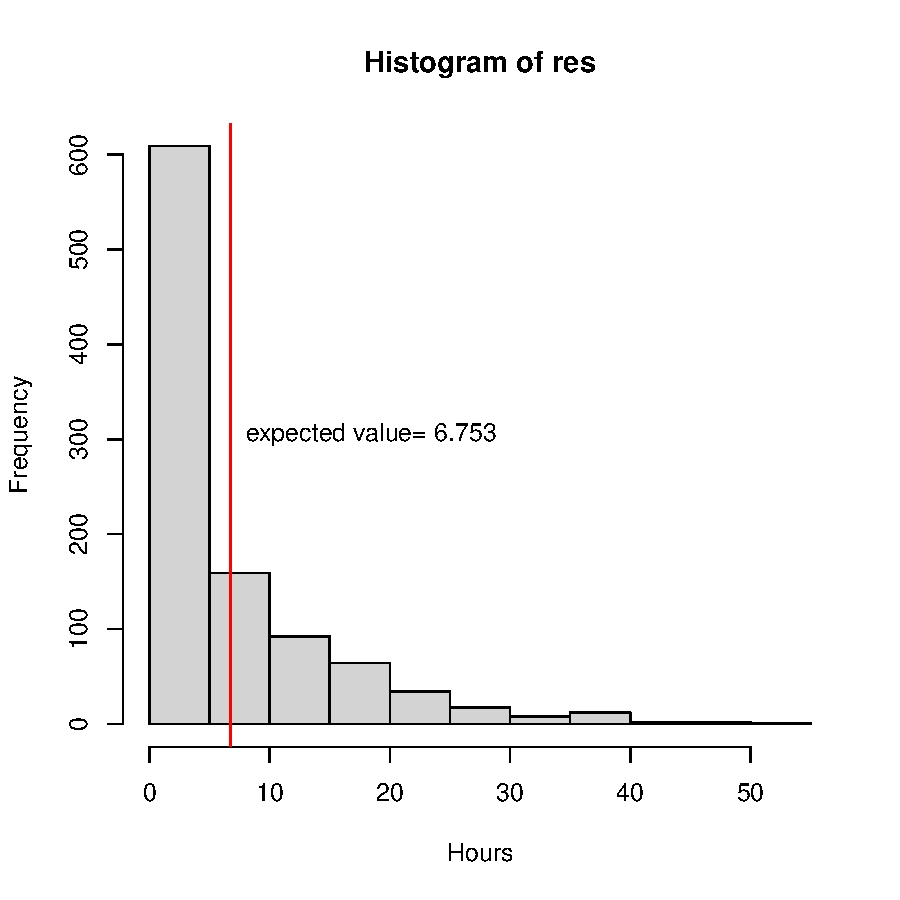
\includegraphics{sim_prisoner_problem-003}


%%%%%%%%%%%%%%%%%%%%%%%%%%%%%%%%%%%%%%%%%%%%%%%%%%%%%%%%%%%%%%%%%%%%%%%%%%%%%%%
